\documentclass[a4paper,11pt]{article}
\usepackage[utf8]{inputenc}
\usepackage{geometry}
\geometry{left = 4.0cm, right = 4.0cm, top = 4.0cm, bottom = 3.5cm}
\usepackage[onehalfspacing]{setspace} 
\usepackage{graphicx}
\usepackage{tabularx}
\usepackage{hyperref}
\usepackage{float} 
\usepackage{ragged2e} %%blocksatz \justifing
\usepackage{minted}
\usepackage[english]{babel} % 将语言改为英文
\usepackage[babel,english=american]{csquotes} % 设置英文引号样式
\usepackage[backend=biber, style=apa]{biblatex} 
\newcommand{\showfontsize}{{\f@size pt}}
% \addbibresource{literature.bib}
\setlength{\bibitemsep}{1em}
\hypersetup{
    colorlinks=true,
    linkcolor=black,     % 目录链接颜色
}

%%%%%%%%%%%%%%%%%%%%%%%%%%%%%%%%%%%%%%%%%%%%%%%%%%%%%%
% Title Page
%%%%%%%%%%%%%%%%%%%%%%%%%%%%%%%%%%%%%%%%%%%%%%%%%%%%%%%
% \documentclass{article}
\usepackage[utf8]{inputenc}
% \usepackage[a4paper, margin=1in]{geometry}
\usepackage{titling} 

% 设置标题页格式
\pretitle{\begin{center}\Huge\bfseries}
\posttitle{\par\end{center}\vspace{2cm}}
\preauthor{\begin{center}\Large}
\postauthor{\par\end{center}\vspace{2cm}}
\predate{\begin{center}\Large}
\postdate{\par\end{center}}

% 计算垂直间距使内容均匀分布
\renewcommand{\maketitlehooka}{%
  \setlength{\droptitle}{-5cm} % 调整标题起始位置
  \vspace*{\fill} % 顶部填充
}
\renewcommand{\maketitlehookd}{%
  \vspace*{\fill} % 底部填充
}

\begin{document}

\title{COMP3314 Assignment 3 \\ Image Classification Report}
\author{
    Team name: 99\% \\
    \vspace{0.5cm} 
    Chen Yuxuan 3036128028\\
    Li Yufei 3036128432\\
    Liu Yantong 3036127012
}
\date{\today}

\maketitle
\newpage
%%%%%%%%%%%%%%%%%%%%%%%%%%%%%%%%%%%%%%%%%%%%%%%%%%%%
% Table of Contents
%%%%%%%%%%%%%%%%%%%%%%%%%%%%%%%%%%%%%%%%%%%%%%%%%%%%%
\tableofcontents
\newpage
%%%%%%%%%%%%%%%%%%%%%%%%%%%%%%%%%%%%%%%%%%%%%%%%%%%
% Abstract
%%%%%%%%%%%%%%%%%%%%%%%%%%%%%%%%%%%%%%%%%%%%%%%%%%%
\section*{Abstract}


%%%%%%%%%%%%%%%%%%%%%%%%%%%%%%%%%%%%%%%%%%%%%%%%%%%
% Dataset Analysis
%%%%%%%%%%%%%%%%%%%%%%%%%%%%%%%%%%%%%%%%%%%%%%%%%%%
\section{Dataset Analysis}
In this section, we present an overview of the dataset, analyzing the statistics on the number of categories. Additionally, we will visualize representative examples from each category to illustrate the diversity and characteristics inherent within the dataset. This analysis aims to provide a foundational understanding of the dataset's structure, which is essential for subsequent modeling and interpretation.

\subsection{Load Data}
We load the data and subsequently convert both the training and testing datasets into NumPy arrays, which are easier for our model to process.

\begin{listing}[!ht]
\begin{minted}{python}
csv_path, csv_test_path = "./data/train.csv", "./data/test.csv"
img_dir, img_dir_test = "./data/train_ims", "./data/test_ims"
data_train = pd.read_csv(csv_path)
data_test = pd.read_csv(csv_test_path)
X_train, y_train, X_test, y_test = [], [], [], []

for _, row in data_train.iterrows():
    img_path = os.path.join(img_dir, row.iloc[0])
    label = int(row.iloc[1])
    img = Image.open(img_path).convert("RGB")
    img = np.array(img).flatten()
    X_train.append(img)
    y_train.append(label)

for _, row in data_test.iterrows():
    img_path = os.path.join(img_dir_test, row.iloc[0])
    label = int(row.iloc[1])
    img = Image.open(img_path).convert("RGB")
    img = np.array(img).flatten()
    X_test.append(img)
    y_test.append(label)

X_train, y_train = np.array(X_train), np.array(y_train)
X_test, y_test = np.array(X_test), np.array(y_test)
X_train_flatten = X_train.reshape(X_train.shape[0], -1)
X_test_flatten = X_test.reshape(X_test.shape[0], -1)
\end{minted}
\caption{Load Data}
\label{listing:python}
\end{listing}

\subsection{Statistics on the number of categories}

\subsubsection{Dataset Size}

\begin{listing}[!ht]
\begin{minted}{python}
print("The shape of the training set: ", X_train.shape)
print("The shape of the testing set: ", X_test.shape)
print("Training set (flattened): ", X_train_flatten.shape)
print("Testing set (flattened): ", X_test_flatten.shape)
print("The size of the label of the training set: ", y_train.shape)
print("The size of the label of the testing set: ", y_test.shape)
\end{minted}
\caption{Print the shape of the datasets}
\label{listing:python}
\end{listing}

\begin{itemize}
    \item \textbf{Size Statistics}
    \item The shape of the training set: \textbf{(50000, 32, 32, 3)}
    \item The shape of the testing set: \textbf{(10000, 32, 32, 3)}
    \item Training set (flattened): \textbf{(50000, 3072)}
    \item Testing set (flattened): \textbf{(10000, 3072)}
    \item The size of the label of the training set:  \textbf{(50000,)}
    \item The size of the label of the test set: \textbf{(10000,)}
\end{itemize}

\subsubsection{Category Label Count}

\begin{listing}[!ht]
\begin{minted}{python}
# Count the labels
count_labels = np.unique(y_train, return_counts=True)

# Create DataFrame
label_counts_df = pd.DataFrame({
    "Label": count_labels[0],
    "Count": count_labels[1]
}).set_index("Label")

# Print DataFrame
print("Count of each label:")
print(label_counts_df)
\end{minted}
\caption{Count the number of each category}
\label{listing:python}
\end{listing}

\begin{table}[h]
    \centering
    \begin{tabular}{|c|c|c|c|c|}
        \hline
        Label 0 & Label 1 & Label 2 & Label 3 & Label 4 \\
        \hline
        \textbf{5038} & \textbf{5016} & \textbf{5032} & \textbf{4991} & \textbf{4982} \\
        \hline
        Label 5 & Label 6 & Label 7 & Label 8 & Label 9 \\
        \hline
        \textbf{4967} & \textbf{4985} & \textbf{4998} & \textbf{5002} & \textbf{4989} \\
        \hline
    \end{tabular}
    \caption{Label Counts in training set}
    \label{tab:example}
\end{table}

\begin{figure}[H]
    \centering
    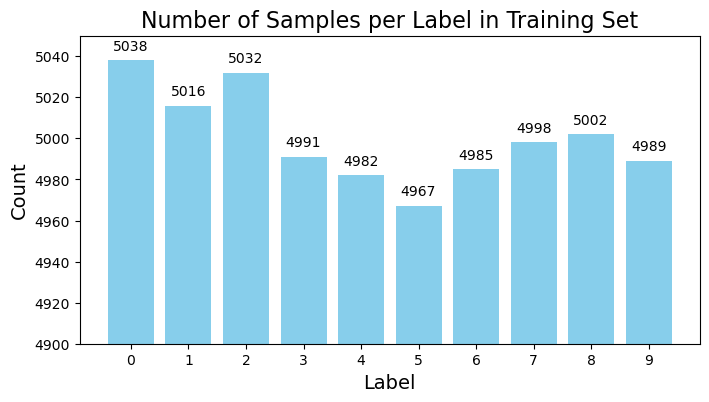
\includegraphics[scale=0.7]{./img/Label_counts.png}
    \caption[Label count] {Label Counts in training set}
\end{figure}

\subsubsection{Other Statistics}

\begin{listing}[!ht]
\begin{minted}{python}
print("Other Statistics for the training set label:")
print(pd.Series(y_train).describe())
\end{minted}
\caption{Print other statistics of the labels of the training set}
\label{listing:python}
\end{listing}

\begin{verbatim}
count    50000.00000
mean         4.49258
std          2.87539
min          0.00000
25%          2.00000
50%          4.00000
75%          7.00000
max          9.00000
\end{verbatim}

\subsection{Image Visualization}
\subsubsection{One Example for Each Category}

\begin{listing}[!ht]
\begin{minted}{python}
def visualize_images_by_label(img_dir, data, y):
    unique_labels = np.unique(y)
    fig, axes = plt.subplots(2, 5, figsize=(15, 6))
    for i, label in enumerate(unique_labels[:10]): 
        indices = np.where(y == label)[0]
        idx = np.random.choice(indices)
        img = Image.open(os.path.join(img_dir, data.iloc[idx, 0]))
        row = i // 5
        col = i % 5
        ax = axes[row, col] 
        ax.imshow(img)
        ax.set_title(f"Label {label}")
        ax.axis('off')
    for j in range(i+1, 10):
        row = j // 5
        col = j % 5
        axes[row, col].axis('off')
    plt.tight_layout()
    plt.savefig("1 example.png", format='png', bbox_inches='tight')
    plt.show()
visualize_images_by_label(img_dir, data_train, y_train)
\end{minted}
\label{listing:python}
\end{listing}

\begin{figure}[H]
    \centering
    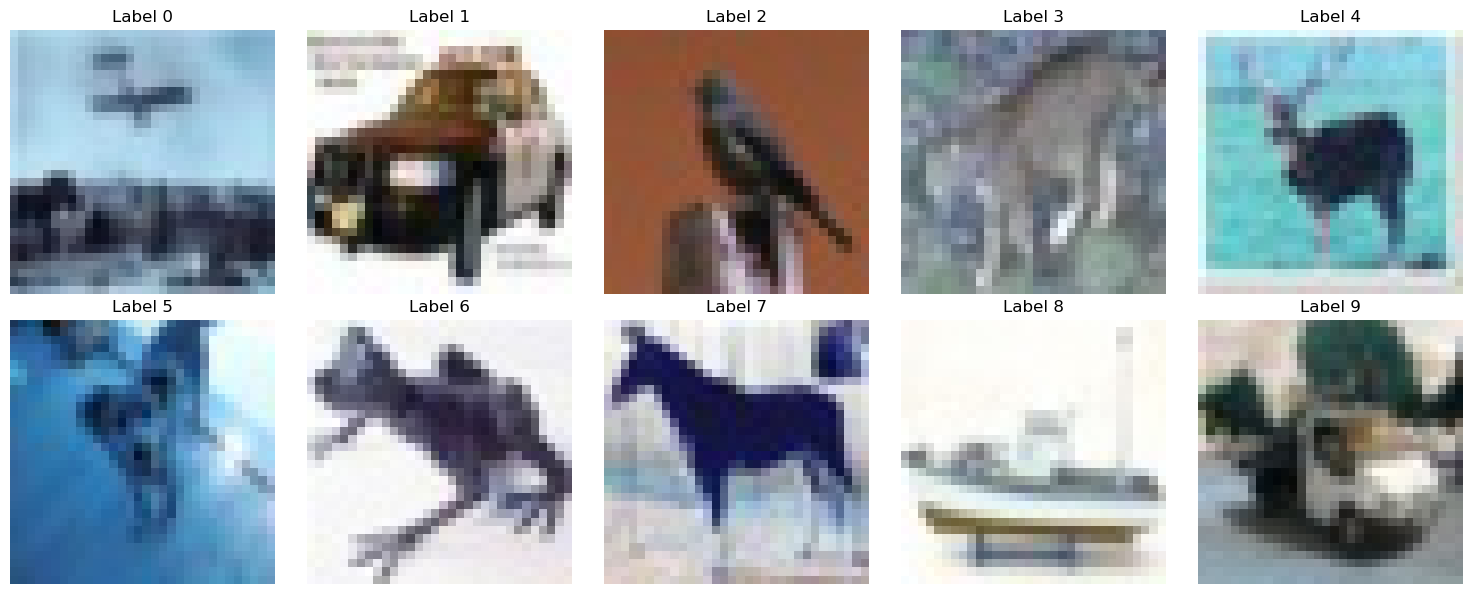
\includegraphics[width=\linewidth]{./img/1 example.png}
    \caption[Label count]{Visualization of one example for each category}
    \label{fig:example}
\end{figure}

\subsubsection{Ten Examples for Each Category}
\begin{listing}[!ht]
\begin{minted}{python}
count_labels = np.unique(y_train, return_counts=True)
label_counts_df = pd.DataFrame({
    "Label": count_labels[0],
    "Count": count_labels[1]
}).set_index("Label")

def get_example_images(label, num_examples=10):
    indices = np.where(y_train == label)[0]
    selected_indices = np.random.choice(indices, 
        size=min(num_examples, len(indices)), replace=False)
    example_images = [os.path.join(img_dir, data_train.iloc[i, 0]) 
        for i in selected_indices]
    return " ".join([f'<img src="{img}" width="50" />' 
        for img in example_images])

label_counts_df["Example Images"] =                               
label_counts_df.index.map(get_example_images)
HTML(label_counts_df.to_html(escape=False))
\end{minted}
\label{listing:python}
\end{listing}

\begin{figure}[H]
    \centering
    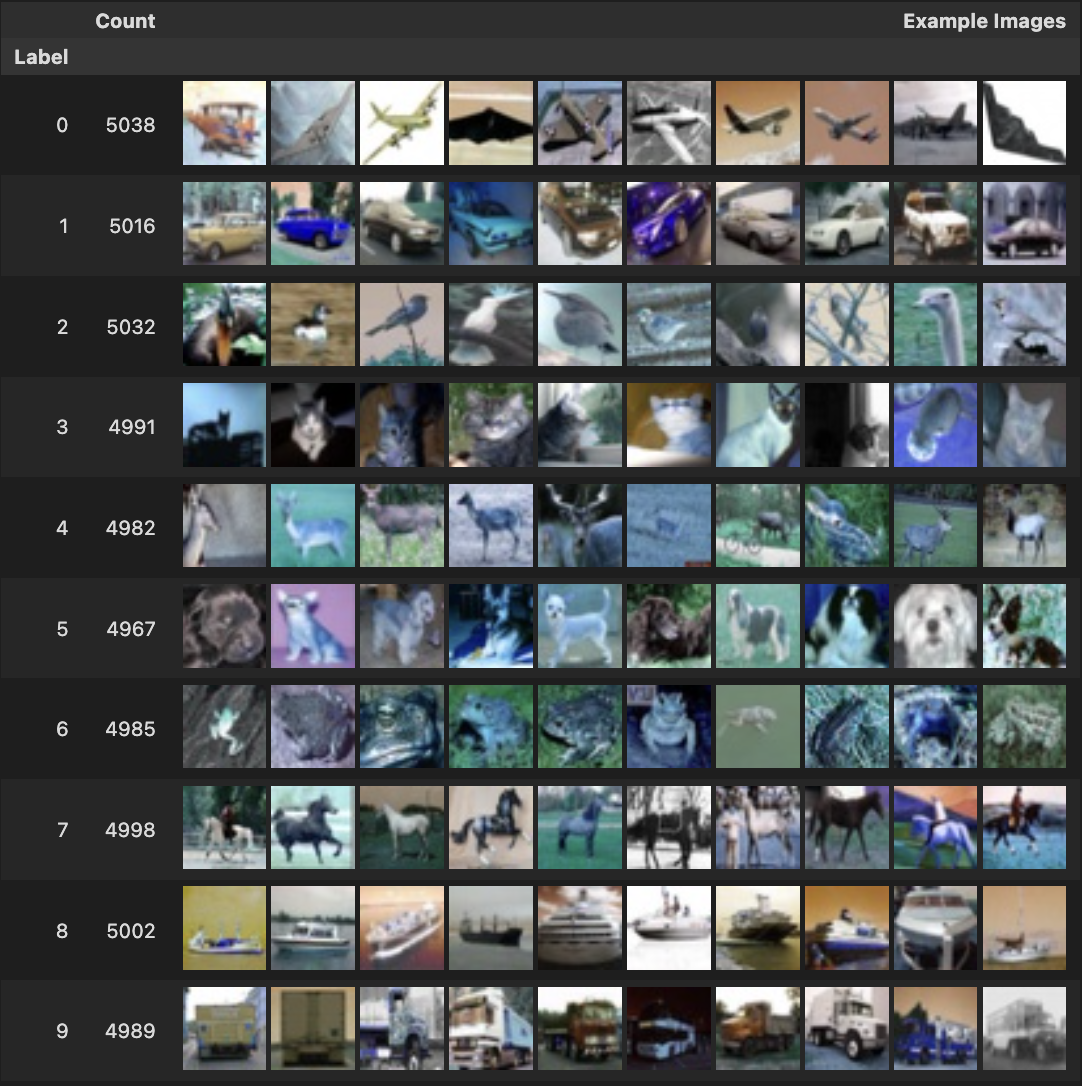
\includegraphics[width=\linewidth]{./img/10 examples.png}
    \caption[Label count]{Visualization of ten example for each category}
    \label{fig:example}
\end{figure}
%%%%%%%%%%%%%%%%%%%%%%%%%%%%%%%%%%%%%%%%%%%%%%%%%%%
% Classifiers Comparison
%%%%%%%%%%%%%%%%%%%%%%%%%%%%%%%%%%%%%%%%%%%%%%%%%%%
\section{Classifiers Comparison}
In this section, we'll explain how we tested and compared three different classifiers: KNN(K Nearest Neighbor), SVM(Support Vector Machine), RF(Random Forest) using the original dataset and the dataset with feature extraction(explained in Section 4).

\subsection{Basic Workflow for testing classifiers}
For the independence of variables, we use the following workflow for each models to ensure that factors such as the training set will not affect the three classifiers. 
\\
In this code, we use Pipeline to manage the process and the classification\_report function of sklearn to estimate the performance, making the code more readable and satisfying the independence of variables.

\begin{minted}{python}
from sklearn.decomposition import PCA
from sklearn.preprocessing import StandardScaler
from sklearn.pipeline import make_pipeline
from sklearn.svm import SVC
from sklearn.metrics import accuracy_score
#%%%%%%%%%%%%%%%%%%%%%%%%%%%%
#build the pipeline
#%%%%%%%%%%%%%%%%%%%%%%%%%%%%
XX_model = make_pipeline(
    StandardScaler(), 
    PCA(n_components=0.75, random_state=SEED), 
    XX())

#%%%%%%%%%%%%%%%%%%%%%%%%%%%%
#Train and predict
#%%%%%%%%%%%%%%%%%%%%%%%%%%%%
XX_model.fit(X_train_featured, y_train_aug)

y_pred_XX = XX_model.predict(X_val_featured)
accuracy_XX = accuracy_score(y_val, y_pred_XX)
from sklearn.metrics import classification_report
from sklearn.metrics import confusion_matrix
from matplotlib import pyplot as plt

#%%%%%%%%%%%%%%%%%%%%%%%%%%%%
#Report
#%%%%%%%%%%%%%%%%%%%%%%%%%%%%
# Classification Report
report = classification_report(y_val, y_pred_XX)

print("Classification Report:")
print(classification_report(y_val, y_pred_XX))

output_file = "classification_report.txt"

with open(output_file, "w") as f:
    f.write("Classification Report:\n")
    f.write(report)

print(f"Classification report saved to {output_file}")
\end{minted}
\subsection{The performance of three classifiers}
The performance of three classifiers with origin data is shown below:
\begin{minted}{bash}
SVM Validation Accuracy: 0.4978
Classification Report:
              precision    recall  f1-score   support
           0       0.53      0.55      0.54      1011
           1       0.58      0.60      0.59      1051
           2       0.38      0.38      0.38       985
           3       0.35      0.33      0.34       983
           4       0.41      0.41      0.41       968
           5       0.44      0.39      0.41       975
           6       0.49      0.59      0.54      1022
           7       0.59      0.55      0.57       987
           8       0.60      0.62      0.61       996
           9       0.58      0.54      0.56      1022
    accuracy                           0.50     10000
   macro avg       0.50      0.50      0.49     10000
weighted avg       0.50      0.50      0.50     10000

KNN Validation Accuracy: 0.4029
Classification Report:
              precision    recall  f1-score   support
           0       0.41      0.57      0.48      1011
           1       0.55      0.40      0.47      1051
           2       0.28      0.38      0.32       985
           3       0.31      0.21      0.25       983
           4       0.28      0.38      0.32       968
           5       0.42      0.26      0.32       975
           6       0.36      0.51      0.42      1022
           7       0.57      0.36      0.44       987
           8       0.49      0.57      0.53       996
           9       0.59      0.36      0.45      1022
    accuracy                           0.40     10000
   macro avg       0.43      0.40      0.40     10000
weighted avg       0.43      0.40      0.40     10000

RF Validation Accuracy: 0.4573
Classification Report:
              precision    recall  f1-score   support
           0       0.53      0.52      0.52      1011
           1       0.50      0.56      0.53      1051
           2       0.40      0.34      0.37       985
           3       0.32      0.29      0.30       983
           4       0.41      0.38      0.39       968
           5       0.38      0.35      0.37       975
           6       0.45      0.51      0.48      1022
           7       0.53      0.47      0.50       987
           8       0.53      0.62      0.57       996
           9       0.48      0.52      0.50      1022
    accuracy                           0.46     10000
   macro avg       0.45      0.46      0.45     10000
weighted avg       0.45      0.46      0.45     10000
\end{minted}

After feature extrations(which will be detailed explained in the following sections), the performance is:
\begin{minted}{bash}
SVM Validation Accuracy: 0.7553
Classification Report:
              precision    recall  f1-score   support
           0       0.79      0.83      0.81      1011
           1       0.87      0.87      0.87      1051
           2       0.65      0.66      0.65       985
           3       0.55      0.56      0.56       983
           4       0.68      0.73      0.70       968
           5       0.64      0.61      0.62       975
           6       0.83      0.81      0.82      1022
           7       0.84      0.80      0.82       987
           8       0.85      0.85      0.85       996
           9       0.85      0.83      0.84      1022
    accuracy                           0.76     10000
   macro avg       0.75      0.75      0.75     10000
weighted avg       0.76      0.76      0.76     10000

KNN Validation Accuracy: 0.5914
Classification Report:
              precision    recall  f1-score   support
           0       0.75      0.65      0.70      1011
           1       0.77      0.81      0.79      1051
           2       0.63      0.41      0.50       985
           3       0.63      0.14      0.23       983
           4       0.42      0.60      0.50       968
           5       0.69      0.26      0.38       975
           6       0.35      0.92      0.51      1022
           7       0.84      0.62      0.72       987
           8       0.72      0.75      0.73       996
           9       0.74      0.70      0.72      1022
    accuracy                           0.59     10000
   macro avg       0.65      0.59      0.58     10000
weighted avg       0.66      0.59      0.58     10000

RF Validation Accuracy: 0.5410
Classification Report:
              precision    recall  f1-score   support
           0       0.59      0.63      0.61      1011
           1       0.65      0.74      0.69      1051
           2       0.45      0.38      0.41       985
           3       0.36      0.26      0.30       983
           4       0.42      0.40      0.41       968
           5       0.42      0.49      0.45       975
           6       0.58      0.66      0.62      1022
           7       0.62      0.59      0.61       987
           8       0.61      0.65      0.63       996
           9       0.62      0.59      0.61      1022
    accuracy                           0.54     10000
   macro avg       0.53      0.54      0.53     10000
weighted avg       0.53      0.54      0.54     10000

\end{minted}
\subsection{Analysis and Final choice}
\textbf{Before Feature Extraction}
\\SVM: Moderate accuracy (~50\%), balanced but mediocre performance.
\\KNN: Poor accuracy (~40\%), high variability across classes.
\\RF: Slightly better (~46\%), but still struggles with some classes.
\\
\\
\textbf{After Feature Extraction}
\\SVM: Best performance (75.5\% accuracy), consistent across all classes.
\\KNN: Improved (~59\%), but suffers from extreme recall imbalances (e.g., some classes <20\%).
\\RF: Minor improvement (~54\%), still lacks robustness in difficult classes.
\\
\\

\subsection{Final Choice}
We select SVM as our final classifier based on two key advantages:

\begin{itemize}
    \item \textbf{Superior Classification Performance}:
    \begin{itemize}
        \item Achieves highest accuracy (75.5\%) among all candidates
        \item Maintains stable performance across all classes (F1-score range: 0.56-0.87)
        \item Demonstrates 25.7\% absolute improvement after feature extraction
    \end{itemize}
    
    \item \textbf{Dimensionality Robustness}:
    \begin{itemize}
        \item Effectively handles high-dimensional feature space
        \item Shows strongest synergy with our feature extraction pipeline
        \item Margin-based optimization prevents overfitting
    \end{itemize}
\end{itemize}
And since SVM excels with enhanced features, adding weaker models (KNN/RF) would add noise, not value. So we didn't ensemble other weaker models.


%%%%%%%%%%%%%%%%%%%%%%%%%%%%%%%%%%%%%%%%%%%%%%%%%%%
% Final Model
%%%%%%%%%%%%%%%%%%%%%%%%%%%%%%%%%%%%%%%%%%%%%%%%%%%
\section{Final Model}

\subsection{Overall Model Structure}
The overall structure of our classification model is as follows. We used data augmentation techniques such as horizontal flipping, random cropping, random rotation, and random color jittering to increase the size of the training dataset to approximately 2.3 times the original. Then, we employed the HOG method, supplemented by SIFT, HIST, EOG, and ORB methods, for feature extraction from the training set, while resizing the features during extraction for finer detail. Finally, We created a pipeline comprising StandardScaler, PCA, and SVM for training.

\subsection{Feature Extraction}

In the feature extraction process, we utilized several methods to extract features from the images. The following sections will detail the feature extraction methods we employed, including HOG, EOG, ORB, HIST, and LBP. We will also provide visualizations of the features extracted by each method.

%------------------HOG---------------------
\subsubsection{HOG (Histogram of oriented gradients)}

The Histogram of Oriented Gradients (HOG) is a feature descriptor widely used in computer vision for object detection. It quantifies local gradient orientations by dividing an image into cells, computing gradient magnitudes and orientations within each cell, and aggregating them into orientation-based histograms. These histograms are normalized within overlapping spatial blocks to enhance illumination invariance. HOG effectively captures edge structure and texture patterns, achieving robustness to geometric and photometric variations.

\begin{figure}[H]
    \centering
    \includegraphics[width=0.7\textwidth]{./img/visual_hog.png}
    \caption[visual_hog] {Visualization of HOG}
\end{figure}

In our implementation, we firstly resize the image to 128x128 pixels, then split the image into three channels (RGB), and finally apply HOG to each channel. The HOG features are concatenated into a single feature vector for each image. The following code demonstrates the process:

\begin{minted}{python}
def HOG_extractor(image, target_size=(128, 128)):
    if len(image.shape) == 1:
        image = image.reshape(32, 32, 3)  # Adjust this based on your original image shape

    resized_img = cv2.resize(image, target_size, interpolation=cv2.INTER_LINEAR)
    channels = cv2.split(resized_img)
    
    hog_kwargs = {
        "_winSize": (128, 128),
        "_blockSize": (64, 64),
        "_blockStride": (16, 16),
        "_cellSize": (16, 16),
        "_nbins": 10,
        "_derivAperture": 1,
        "_winSigma": -1,
        "_histogramNormType": 0,
        "_L2HysThreshold": 0.2,
        "_gammaCorrection": True,
        "_nlevels": 64,
        "_signedGradient": True
    }   

    hog = cv2.HOGDescriptor(**hog_kwargs)

    hog_features = []
    for channel in channels:
        hog_feature = hog.compute(channel)
        hog_features.append(hog_feature.flatten())

    return np.concatenate(hog_features)
\end{minted}

After adopting the HOG method, the performance of the SVM rbf kernel model improved significantly, the average accuracy increased around 20\%.
As a result, we decided to use HOG as our main feature extraction method.

%--------------------EOG---------------------
\subsubsection{EOG (Extract Edge Orientation Gradient)}

The EOG extraction method offers a computationally efficient approach for capturing essential structural information by combining Canny edge detection with gradient analysis, which enhances boundary sensitivity through precise thresholding and Sobel filtering while suppressing noise. Its grayscale conversion and feature vector flattening optimize processing efficiency and storage requirements, while image resizing maintains dimensional consistency across varied inputs. The method simultaneously preserves rich directional texture characteristics through gradient magnitude (quantifying edge strength) and orientation (encoding angular patterns), enabling comprehensive yet compact representation of both geometric contours and subtle surface variations in visual data.

\begin{figure}[H]
    \centering
    \includegraphics[width=0.7\textwidth]{./img/visual_eog.png}
    \caption[visual_hog] {Visualization of EOG}
\end{figure}

After add the EOG, the accuracy increased around 1\% compared to the HOG method, from 0.7670 to 0.7792.

We try both 3 channel EOG and 1 channel EOG, however, the performance of 3 channel EOG is not as good as 1 channel EOG. The following code demonstrates the process.
The accuracy of 3 channel EOG is 0.7787, while the accuracy of 1 channel EOG is around 0.7792.
Therefore, we only use 1 channel EOG as our feature extraction method. We indicate the abnormal result may be caused by overfitting, as the 3 channel EOG has more features than the 1 channel EOG.

The implementation of EOG is as follows:

\begin{minted}{python}
def EOG_extractor(image, target_size=(32, 32)):
    if len(image.shape) == 1:
        image = image.reshape(32, 32, 3)
        
    resized_img = cv2.resize(image, target_size, interpolation=cv2.INTER_CUBIC)
    gray_img = cv2.cvtColor(resized_img, cv2.COLOR_RGB2GRAY)

    # Apply Canny edge detection
    edges = cv2.Canny(gray_img, threshold1=100, threshold2=200)
    # Compute gradients in x and y directions
    grad_x = cv2.Sobel(edges, cv2.CV_64F, 1, 0, ksize=3)
    grad_y = cv2.Sobel(edges, cv2.CV_64F, 0, 1, ksize=3)
    # Compute gradient magnitude and orientation
    magnitude = np.sqrt(grad_x**2 + grad_y**2)
    orientation = np.arctan2(grad_y, grad_x)
    # Flatten the magnitude and orientation into a feature vector
    eog_feature = np.concatenate([magnitude.flatten(), orientation.flatten()])

    return eog_feature
\end{minted}

Meanwhile, the effect of EOG feature extraction on resized images is not satisfactory, which reduces the final accuracy by 1\%, drop to 0.7655. 

%--------------------ORB--------------------
\subsubsection{ORB(Oriented FAST and Rotated BRIEF)}

ORB is a fast and efficient feature extraction algorithm used in computer vision. It combines the FAST keypoint detector, which identifies keypoints based on intensity changes, with the BRIEF descriptor, which encodes local image patches into binary strings for matching. ORB introduces improvements such as orientation estimation for rotation invariance and a more robust descriptor through rotated BRIEF.

\begin{figure}[H]
    \centering
    \includegraphics[width=0.7\textwidth]{./img/visual_orb.png}
    \caption[visual_hog] {Visualization of ORB}
\end{figure}

We try to use the ORB as our supplementary feature extraction method. The implementation of ORB is as follows:

\begin{minted}{python}
def ORB_extractor(image, target_size=(256, 256), n_features=500, fixed_length=1000):
    orb = cv2.ORB_create(nfeatures=n_features)
    if len(image.shape) == 1:
        image = image.reshape(32, 32, 3)
    resized_img = cv2.resize(image, target_size, interpolation=cv2.INTER_CUBIC)
    gray_img = cv2.cvtColor(resized_img, cv2.COLOR_RGB2GRAY)

    # Detect keypoints and compute descriptors
    keypoints, descriptors = orb.detectAndCompute(gray_img, None)
    # If no descriptors are found, return a zero vector
    if descriptors is None:
        descriptors = np.zeros((1, 32), dtype=np.uint8)

    descriptors = descriptors.flatten()
    if len(descriptors) < fixed_length:
        descriptors = np.pad(descriptors, (0, fixed_length - len(descriptors)), mode='constant')
    elif len(descriptors) > fixed_length:
        descriptors = descriptors[:fixed_length]

    return descriptors.flatten()
\end{minted}

However, the ORB feature extraction process has become a performance bottleneck, degrading the overall accuracy by around 1\%.

%--------------------HIST--------------------
\subsubsection{HIST(Histogram of Intensity and Surface Texture)}

The Histogram of Intensity and Surface Texture (HIST) feature extraction method quantifies spatial-intensity distributions and textural patterns by constructing multi-dimensional histograms across localized image regions. It employs adaptive binning to capture intensity gradients and co-occurrence statistics, coupled with spatial pooling to preserve structural context. Normalization techniques mitigate illumination variations while entropy-based weighting enhances discriminative power. This approach balances computational efficiency with robustness to affine transformations, making it particularly effective for texture classification, material recognition, and illumination-invariant object detection in computer vision application

\begin{figure}[H]
    \centering
    \includegraphics[width=0.7\textwidth]{./img/visual_hist.png}
    \caption[visual_hog] {Visualization of ORB}
\end{figure}

Our implementation is based on the OpenCV library, which provides a convenient function for histogram calculation. The following code demonstrates the process:

\begin{minted}{python}
def HIST_extractor(image, target_size=(256, 256), bins=(8, 8, 8)):
    if len(image.shape) == 1:
        image = image.reshape(32, 32, 3)
    resized_img = cv2.resize(image, target_size, interpolation=cv2.INTER_LINEAR)
    
    # Compute the color histogram for each channel (B, G, R)
    hist = cv2.calcHist([resized_img], [0, 1, 2], None, bins, [0, 256, 0, 256, 0, 256])
    # Normalize the histogram
    hist = cv2.normalize(hist, hist).flatten()

    return hist
\end{minted}

By adding the HIST method, the accuracy increased around 1\% compared to the single EOG + HOG method, from 0.7670 to 0.7792.

%--------------------LBP--------------------
\subsubsection{LBP (Local Binary Patterns)}

The Local Binary Patterns (LBP) method encodes texture information by comparing pixel intensities with their circular neighborhood.

\begin{figure}[H]
    \centering
    \includegraphics[width=0.7\textwidth]{./img/visual_lbp_methods.png}
    \caption[visual_hog] {Visualization of ORB}
\end{figure}

Our OpenCV-based implementation adopts uniform pattern mapping with histogram normalization:

\begin{minted}{python}
def LBP_extractor(image, target_size=(64, 64)):
    if len(image.shape) == 1:
        image = image.reshape(32, 32, 3)  # Adjust this based on your original image shape
    resized_img = cv2.resize(image, target_size, interpolation=cv2.INTER_LINEAR)

    # Convert to grayscale
    gray_img = rgb2gray(resized_img)
    # Compute LBP features
    lbp = local_binary_pattern(gray_img, P=8, R=1, method='default')
    # Flatten the LBP feature vectorq
    return lbp.flatten()
\end{minted}

While theoretically effective for texture characterization, our implementation exhibited around 1.3\% accuracy drop (from 0.7792 to 0.7668) when integrated into the feature ensemble (both deafult and uniform lbp), suggesting potential implementation challenges or feature conflicts.

%-------------------SIFT---------------------
\subsubsection{SIFT(Scale-Invariant Feature Transform)}

SIFT detects and describes distinctive image features invariant to scale, rotation, and illumination by: 1) Identifying keypoints via Difference-of-Gaussians extrema in scale-space pyramids; 2) Assigning orientation-based descriptors using gradient orientation histograms in localized regions. Its 128-dimensional vectors enable robust matching for object recognition, 3D reconstruction, and image alignment despite viewpoint changes or partial occlusion.

\begin{figure}[H]
    \centering
    \includegraphics[width=0.7\textwidth]{./img/visual_sift.png}
    \caption[visual_hog] {Visualization of ORB}
\end{figure}

Our implementation is as follows:

\begin{minted}{python}
def SIFT_extractor(image, n_features=128):
    sift = cv2.SIFT_create()
    if not isinstance(image, np.ndarray):
        image = np.array(image)
    if len(image.shape) == 1:
        image = image.reshape(32, 32, 3) 

    channels = cv2.split(image)
    descriptors_list = []
    
    for channel in channels:
        keypoints, descriptors = sift.detectAndCompute(channel, None)
        # If no descriptors are found, return an empty array
        if descriptors is None:
            descriptors = np.zeros((1, n_features)).flatten()
        descriptors_mean = np.mean(descriptors, axis=0)
        descriptors_list.append(descriptors_mean)
        
    combined_descriptors = np.concatenate(descriptors_list)

    return combined_descriptors
\end{minted}

However, adding the SIFT has no significant effect on the accuracy, which is around 0.7792.
To save more memory for the training process, we decided to remove the SIFT method from our final model.

%--------------------LYF--------------------
% \subsubsection{HOG (Histogram of oriented gradients)}

% The Histogram of Oriented Gradients (HOG) is a feature descriptor widely used in computer vision for object detection. It quantifies local gradient orientations by dividing an image into cells, computing gradient magnitudes and orientations within each cell, and aggregating them into orientation-based histograms. These histograms are normalized within overlapping spatial blocks to enhance illumination invariance. HOG effectively captures edge structure and texture patterns, achieving robustness to geometric and photometric variations.

% \begin{minted}{python}
% def HOG_extractor(image, target_size=(128, 128)):
%     if len(image.shape) == 1:
%         image = image.reshape(32, 32, 3)  # Adjust this based on your original image shape

%     resized_img = cv2.resize(image, target_size, interpolation=cv2.INTER_LINEAR)
%     channels = cv2.split(resized_img)
    
%     hog_kwargs = {
%         "_winSize": (128, 128),
%         "_blockSize": (64, 64),
%         "_blockStride": (16, 16),
%         "_cellSize": (16, 16),
%         "_nbins": 10,
%         "_derivAperture": 1,
%         "_winSigma": -1,
%         "_histogramNormType": 0,
%         "_L2HysThreshold": 0.2,
%         "_gammaCorrection": True,
%         "_nlevels": 64,
%         "_signedGradient": True
%     }   

%     hog = cv2.HOGDescriptor(**hog_kwargs)

%     hog_features = []
%     for channel in channels:
%         hog_feature = hog.compute(channel)
%         hog_features.append(hog_feature.flatten())

%     return np.concatenate(hog_features)
% \end{minted}

% \begin{figure}[H]
%     \centering
%     \includegraphics[width=\linewidth]{./img/visual_hog.png}
%     \caption[Label count]{Visualization of HOG}
%     \label{fig:example}
% \end{figure}

% \subsubsection{EOG (Extract Edge Orientation Gradient)}

% EOG is a feature descriptor that captures the geometric layout of prominent edges in an image by analyzing their orientation distribution. The image is divided into uniform grid cells, where the dominant edge orientations within each cell are detected and encoded into a directional frequency matrix. By integrating multi-scale grid fusion and orientation consistency verification, EOG effectively represents the contour topology of objects while maintaining robustness to local deformations and viewpoint variations. Its sparse encoding mechanism ensures high computational efficiency, making it suitable for real-time edge-based scene matching and object recognition tasks.

% \begin{minted}{python}
% def EOG_extractor(image, target_size=(32, 32)):
%     """
%     Extract Edge Orientation Gradient (EOG) features from a single image.

%     Parameters:
%         image (numpy.ndarray): Input image, shape (H, W, C) or (H*W*C).
%         target_size (tuple): Target size to resize the image before extracting EOG features.

%     Returns:
%         numpy.ndarray: Flattened EOG feature vector for the input image.
%     """
%     if len(image.shape) == 1:
%         image = image.reshape(32, 32, 3)
        
%     # Resize the image to the target size
%     resized_img = cv2.resize(image, target_size, interpolation=cv2.INTER_CUBIC)
    
%     ###############################GRAY###############################
%     # Convert to grayscale
%     gray_img = cv2.cvtColor(resized_img, cv2.COLOR_RGB2GRAY)
%     # Apply Canny edge detection
%     edges = cv2.Canny(gray_img, threshold1=100, threshold2=200)
%     # Compute gradients in x and y directions
%     grad_x = cv2.Sobel(edges, cv2.CV_64F, 1, 0, ksize=3)
%     grad_y = cv2.Sobel(edges, cv2.CV_64F, 0, 1, ksize=3)
%     # Compute gradient magnitude and orientation
%     magnitude = np.sqrt(grad_x**2 + grad_y**2)
%     orientation = np.arctan2(grad_y, grad_x)
%     # Flatten the magnitude and orientation into a feature vector
%     eog_feature = np.concatenate([magnitude.flatten(), orientation.flatten()])

%     return eog_feature
% \end{minted}

% \begin{figure}[H]
%     \centering
%     \includegraphics[width=\linewidth]{./img/eog_output.png}
%     \caption[Label count]{Visualization of EOG}
%     \label{fig:example}
% \end{figure}
% \subsubsection{HIST (Hierarchical Intensity Statistics)}
% HIST is a feature representation method based on hierarchical statistical analysis of color or intensity distributions. The image is decomposed into multi-resolution sub-regions, where localized intensity/chromatic histograms are computed at each scale and aggregated across a Gaussian pyramid. Adaptive histogram equalization mitigates illumination biases, while spatial weighting emphasizes salient object regions. HIST further characterizes texture patterns using higher-order statistical moments (e.g., skewness, kurtosis) to describe micro-intensity distributions. This multi-scale, moment-driven approach demonstrates strong discriminative power for material classification and saliency detection, even in cluttered backgrounds.
% \begin{minted}{python}
% def HIST_extractor(image, target_size=(64, 64), bins=(8, 8, 8)):
%     """
%     Extract color histogram (HIST) features from a single image.

%     Parameters:
%         image (numpy.ndarray): Input image, shape (H, W, C) or (H*W*C).
%         target_size (tuple): Target size to resize the image before extracting HIST features.
%         bins (tuple): Number of bins for each color channel (e.g., (8, 8, 8)).

%     Returns:
%         numpy.ndarray: Flattened HIST feature vector for the input image.
%     """

%     if len(image.shape) == 1:
%         image = image.reshape(32, 32, 3)

%     # Resize the image to the target size
%     resized_img = cv2.resize(image, target_size, interpolation=cv2.INTER_LINEAR)
%     # Compute the color histogram for each channel (B, G, R)
%     hist = cv2.calcHist([resized_img], [0, 1, 2], None, bins, [0, 256, 0, 256, 0, 256])
%     # Normalize the histogram
%     hist = cv2.normalize(hist, hist).flatten()

%     return hist
% \end{minted}

% \begin{figure}[H]
%     \centering
%     \includegraphics[width=\linewidth]{./img/hist_output.png}
%     \caption[Label count]{Visualization of HIST}
%     \label{fig:example}
% \end{figure}

\subsubsection{HSV (Hue-Saturation-Value)}
The Hue-Saturation-Value (HSV) color model is a key tool in computer vision for color-based analysis. It represents colors through three components: Hue (color type, 0°-360°), Saturation (color purity, 0\%-100\%), and Value (brightness, 0\%-100\%). Unlike RGB, HSV separates color information from intensity, making it more robust to lighting changes. This separation allows for effective color segmentation and object detection while maintaining intuitive color manipulation. HSV's perceptual alignment with human vision and its illumination invariance make it particularly useful for applications like skin detection and traffic sign recognition.

\begin{figure}[H]
    \centering
    \includegraphics[width=\linewidth]{./img/hsv_output.png}
    \caption[Label count]{Visualization of HSV}
    \label{fig:example}
\end{figure}


\subsection{Data Augmentation}
As we are restricted to using other data sets, we enhance the training set by processing the training images in the existing data set. In our final model, we applied horizontal flipping to each image, along with a 26×26 crop at the four corners and the center. For each image, there is a probability of 0.1 to perform a random local crop, with the crop size ranging from 24x24 to 32x32 and the crop position being random. Furthermore, there is a probability of 0.1 to apply a random image rotation, with a maximum angle of ±18 degrees. There is also a probability of 0.1 that random color jittering will occur. If color jittering is applied, the brightness, contrast, and hue are randomly adjusted within the range of 0.8 to 1.2.
\subsubsection{Horizontal Flip}
Horizontal flipping is a simple yet effective augmentation technique. By mirroring the images along the vertical axis, we can create a new version of each image. This is particularly useful in scenarios where the orientation of objects is not fixed (e.g., animals, cars, etc.). Since many visual patterns remain unchanged under horizontal flipping, this technique helps our model learn to recognize features regardless of their orientation.

\begin{listing}[!ht]
\begin{minted}{python}
flipped_img = pil_img.transpose(Image.FLIP_LEFT_RIGHT)
\end{minted}
\caption{Horizontal Flips}
\label{listing:python}
\end{listing}

\begin{figure}[ht]
    \centering
    \begin{minipage}{0.49\textwidth}
        \includegraphics[width=\linewidth]{img/original_0.png}
    \end{minipage}
    \hfill
    \begin{minipage}{0.49\textwidth}
        \includegraphics[width=\linewidth]{img/flipped_0.png}
    \end{minipage}
    \caption{[Left]Original [Right]Horizontal Flip}
\end{figure}

\subsubsection{Random Crop}
Random local cropping involves selecting a random portion of the image. With a probability of 0.1, we crop images to sizes between 24x24 and 32x32 pixels (recovered to 32x32 pixels at the end):
\begin{itemize}
    \item \textbf{Crop Size:} By varying the crop size, we expose the model to different scales of the same object, which can help it become invariant to changes in scale.
    \item \textbf{Random Position:} The crop position is also random, ensuring that the model learns to identify relevant features regardless of their location within the image. This simulates the presence of objects at different positions and reinforces the model's ability to generalize.
\end{itemize}

\begin{listing}[!ht]
\begin{minted}{python}
def random_crop(image, crop_size):
    width, height = image.size
    left = random.randint(0, width - crop_size)
    upper = random.randint(0, height - crop_size)
    right = left + crop_size
    lower = upper + crop_size
    return image.crop((left, upper, right, lower))
\end{minted}
\caption{Random Crop}
\label{listing:python}
\end{listing}

\begin{figure}[ht]
    \centering
    \begin{minipage}{0.49\textwidth}
        \includegraphics[width=\linewidth]{img/original_9.png}
    \end{minipage}
    \hfill
    \begin{minipage}{0.49\textwidth}
        \includegraphics[width=\linewidth]{img/cropped_9.png}
    \end{minipage}
    \caption{[Left]Original [Right]Crop}
\end{figure}

\subsubsection{Random Rotation}
Random rotation adds another layer of variability by slightly rotating images within a maximum angle of ±18 degrees. Many objects can appear at various angles in real-world scenarios. By allowing the model to see rotated images, it learns to recognize patterns and features even when they are not perfectly aligned. The rotation is kept within ±18 degrees to prevent excessive distortion, which could lead to loss of important features or misinterpretation of the image content.

\begin{listing}[!ht]
\begin{minted}{python}
def random_rotation(image, max_angle=18):
    angle = random.randint(-max_angle, max_angle)
    return image.rotate(angle)
\end{minted}
\caption{Random Rotation}
\label{listing:python}
\end{listing}

\begin{figure}[ht]
    \centering
    \begin{minipage}{0.49\textwidth}
        \includegraphics[width=\linewidth]{img/original_11.png}
    \end{minipage}
    \hfill
    \begin{minipage}{0.49\textwidth}
        \includegraphics[width=\linewidth]{img/rotated_11.png}
    \end{minipage}
    \caption{[Left]Original [Right]Rotation}
\end{figure}

\subsubsection{Random Color Jittering}
Color jittering introduces variability in the color properties of the images. This technique is particularly useful in real-world scenarios where lighting conditions can vary significantly. 
\begin{itemize}
    \item \textbf{Brightness Adjustment:} Randomly altering the brightness helps the model learn to identify objects under different lighting conditions. 
    \item \textbf{Contrast Adjustment:} Modifying contrast allows the model to become robust against color variations, ensuring it recognizes objects regardless of their color intensity.
    \item \textbf{Hue Adjustment:} Random changes in hue help the model adapt to different color representations of the same object.
\end{itemize}
By adjusting these properties within the range of 0.8 to 1.2, we ensure that the changes are subtle enough to maintain the integrity of the original image.

\begin{listing}[!ht]
\begin{minted}{python}
def color_jitter(image, brightness=0.2, contrast=0.2, color=0.2):
    # Adjust brightness
    enhancer = ImageEnhance.Brightness(image)
    factor = random.uniform(1 - brightness, 1 + brightness)
    image = enhancer.enhance(factor)
    # Adjust contrast
    enhancer = ImageEnhance.Contrast(image)
    factor = random.uniform(1 - contrast, 1 + contrast)
    image = enhancer.enhance(factor)
    # Adjust color
    enhancer = ImageEnhance.Color(image)
    factor = random.uniform(1 - color, 1 + color)
    image = enhancer.enhance(factor)
    return image
\end{minted}
\caption{Random Color Jittering}
\label{listing:python}
\end{listing}

\begin{figure}[ht]
    \centering
    \begin{minipage}{0.49\textwidth}
        \includegraphics[width=\linewidth]{img/original_2.png}
    \end{minipage}
    \hfill
    \begin{minipage}{0.49\textwidth}
        \includegraphics[width=\linewidth]{img/jittered_2.png}
    \end{minipage}
    \caption{[Left]Original [Right]Color Jittering}
\end{figure}

\subsubsection{Approximate Final Size}
The following is the data volume after a certain instance of data augmentation.

\begin{table}[h]
    \centering
    \begin{tabular}{|c|c|c|c|c|}
        \hline
        Label 0 & Label 1 & Label 2 & Label 3 & Label 4 \\
        \hline
        \textbf{11603} & \textbf{11560} & \textbf{11570} & \textbf{11470} & \textbf{11425} \\
        \hline
        Label 5 & Label 6 & Label 7 & Label 8 & Label 9 \\
        \hline
        \textbf{11457} & \textbf{11477} & \textbf{11494} & \textbf{11494} & \textbf{11467} \\
        \hline
    \end{tabular}
    \caption{Label Counts in training set (After augmentation)}
    \label{tab:example}
\end{table}

\begin{verbatim}
Augmented training set shape:  (115017, 3072)
Augmented training set labels shape:  (115017,)
\end{verbatim}

\subsection{StandardScaler}
StandardScaler is used to standardize the features of the dataset by transforming them to have a mean of zero and a standard deviation of one. This normalization is crucial because it ensures that all features contribute equally to the model's performance. Without standardization, features on larger scales may dominate the learning process, leading to suboptimal model performance and slower convergence during training. By applying StandardScaler, we create a balanced dataset that enhances the model's ability to learn from all features effectively.

\subsection{PCA}
Principal Component Analysis (PCA) serves as a dimensionality reduction technique that helps to simplify the dataset while retaining the most significant variance. High-dimensional data can lead to overfitting and increased computational costs. This reduction helps to mitigate the curse of dimensionality, improves computational efficiency, and can also enhance the model's generalization ability.
\begin{itemize}
    \item \textbf{Fine-tuning PCA n\_components}
\end{itemize}
PCA n\_components = 0.8, SVM Validation Accuracy: 0.7789 \\
PCA n\_components = 0.75, SVM Validation Accuracy: 0.7791 \\
PCA n\_components = 0.7, SVM Validation Accuracy: 0.7746 \\
Hence, we choose 0.75 as the n\_components of PCA.

\subsection{SVM Classifier}
From Section 3, we can notice that SVM performs significantly better than other classifiers on this dataset, so we choose not to consider adding other classifiers for ensemble learning and only use SVM.

\begin{listing}[!ht]
\begin{minted}{python}
svm_model = make_pipeline(
    StandardScaler(), 
    PCA(n_components=0.75, random_state=SEED), 
    SVC(C=9, kernel='rbf', gamma='scale',random_state=SEED))

svm_model.fit(X_train_featured, y_train_aug)
\end{minted}
\caption{SVM}
\label{listing:python}
\end{listing}

\begin{itemize}
    \item \textbf{Fine-tuning C}
\end{itemize}
C=6, kernel='rbf', gamma='scale', SVM Validation Accuracy: 0.7788 \\
C=9, kernel='rbf', gamma='scale', SVM Validation Accuracy: 0.7792 \\
C=10, kernel='rbf', gamma='scale', SVM Validation Accuracy: 0.7792 \\
C=12, kernel='rbf', gamma='scale', SVM Validation Accuracy: 0.7792 \\
Hence, we choose C=9 in our SVM model.

\begin{itemize}
    \item \textbf{Fine-tuning kernel}
\end{itemize}
C=9, kernel='rbf', gamma='scale', SVM Validation Accuracy: 0.7792 \\
C=9, kernel='poly', gamma='scale', SVM Validation Accuracy: 0.7587 \\
Hence, we choose kernel='rbf' in our SVM model.

%%%%%%%%%%%%%%%%%%%%%%%%%%%%%%%%%%%%%%%%%%%%%%%%%%%%
% Final Result
%%%%%%%%%%%%%%%%%%%%%%%%%%%%%%%%%%%%%%%%%%%%%%%%%%%%%
\section{Final Result}

\subsection{Performance Analysis}
Using the parameters above, 
We finally achieve a validation accuracy of 80\% and testing accuracy of 80.01\% on kaggle. Our validation result is as follows:
\begin{minted}{python}
Classification Report on Validation Set:
              precision    recall  f1-score   support

           0       0.83      0.86      0.84      1011
           1       0.91      0.89      0.90      1051
           2       0.75      0.71      0.73       985
           3       0.63      0.60      0.61       983
           4       0.73      0.79      0.76       968
           5       0.72      0.65      0.69       975
           6       0.82      0.86      0.84      1022
           7       0.87      0.84      0.86       987
           8       0.87      0.88      0.88       996
           9       0.85      0.91      0.88      1022

    accuracy                           0.80     10000
   macro avg       0.80      0.80      0.80     10000
weighted avg       0.80      0.80      0.80     10000
\end{minted}

\begin{figure}
    \centering
    \includegraphics[width=1\linewidth]{./img/leader_board.png}
    \caption{Kaggle Ranking}
    \label{fig:enter-label}
\end{figure}
\subsection{Future Work}
Based on our confusion matrix analysis, the model demonstrates strong overall performance across most categories. However, there remains room for improvement in distinguishing between label 3 and label 5, as these classes exhibit higher misclassification rates compared to others. To address this, we could implement targeted strategies in subsequent iterations, such as dedicated data augmentation techniques for these two labels (e.g., synthetic sample generation, adversarial training, or class-specific preprocessing). Alternatively, we might explore architectural adjustments like attention mechanisms or loss function modifications to enhance feature discrimination for these challenging pairs. This focused refinement could further optimize the model's precision and robustness in real-world applications.
\begin{figure}
    \centering
    \includegraphics[width=1\linewidth]{img/confusion_matrix_output.png}
    \caption{Confusion Martix}
    \label{fig:enter-label}
\end{figure}


\end{document}